\begin{figure*}[t]
\centering
\begin{subfigure}[t]{0.48\textwidth}
  \centering
  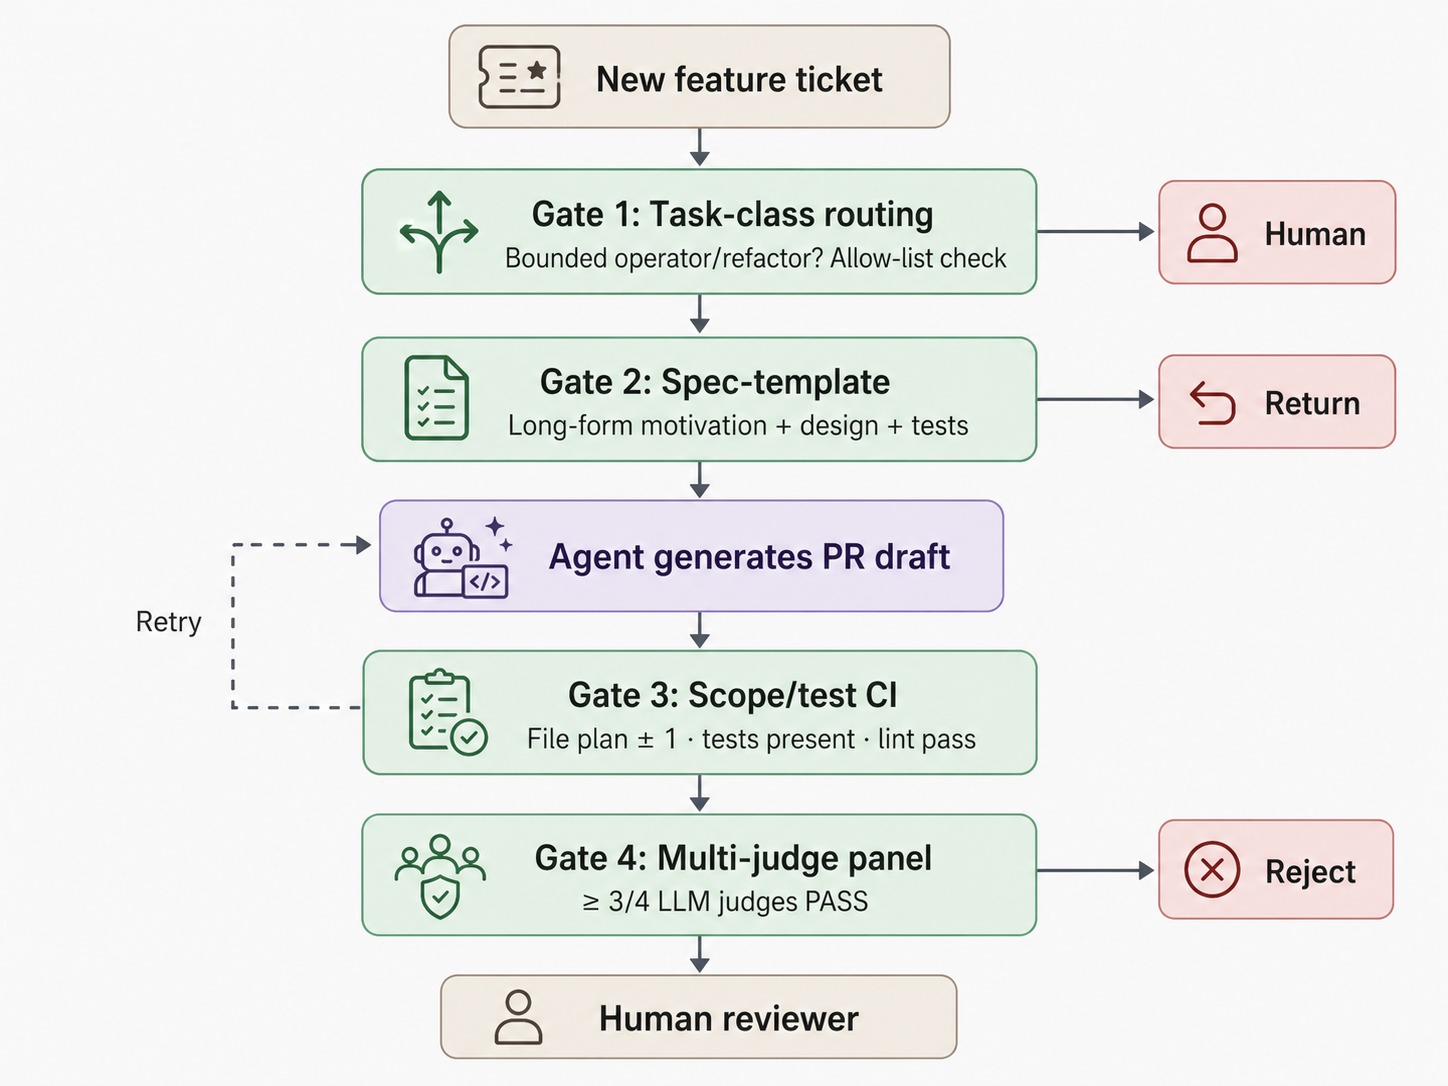
\includegraphics[width=\linewidth]{svg/deployment_gate_pipeline.png}
  \caption{Implication-oriented routing pipeline.}
  \label{fig:deployment-gates}
\end{subfigure}\hfill
\begin{subfigure}[t]{0.48\textwidth}
  \centering
  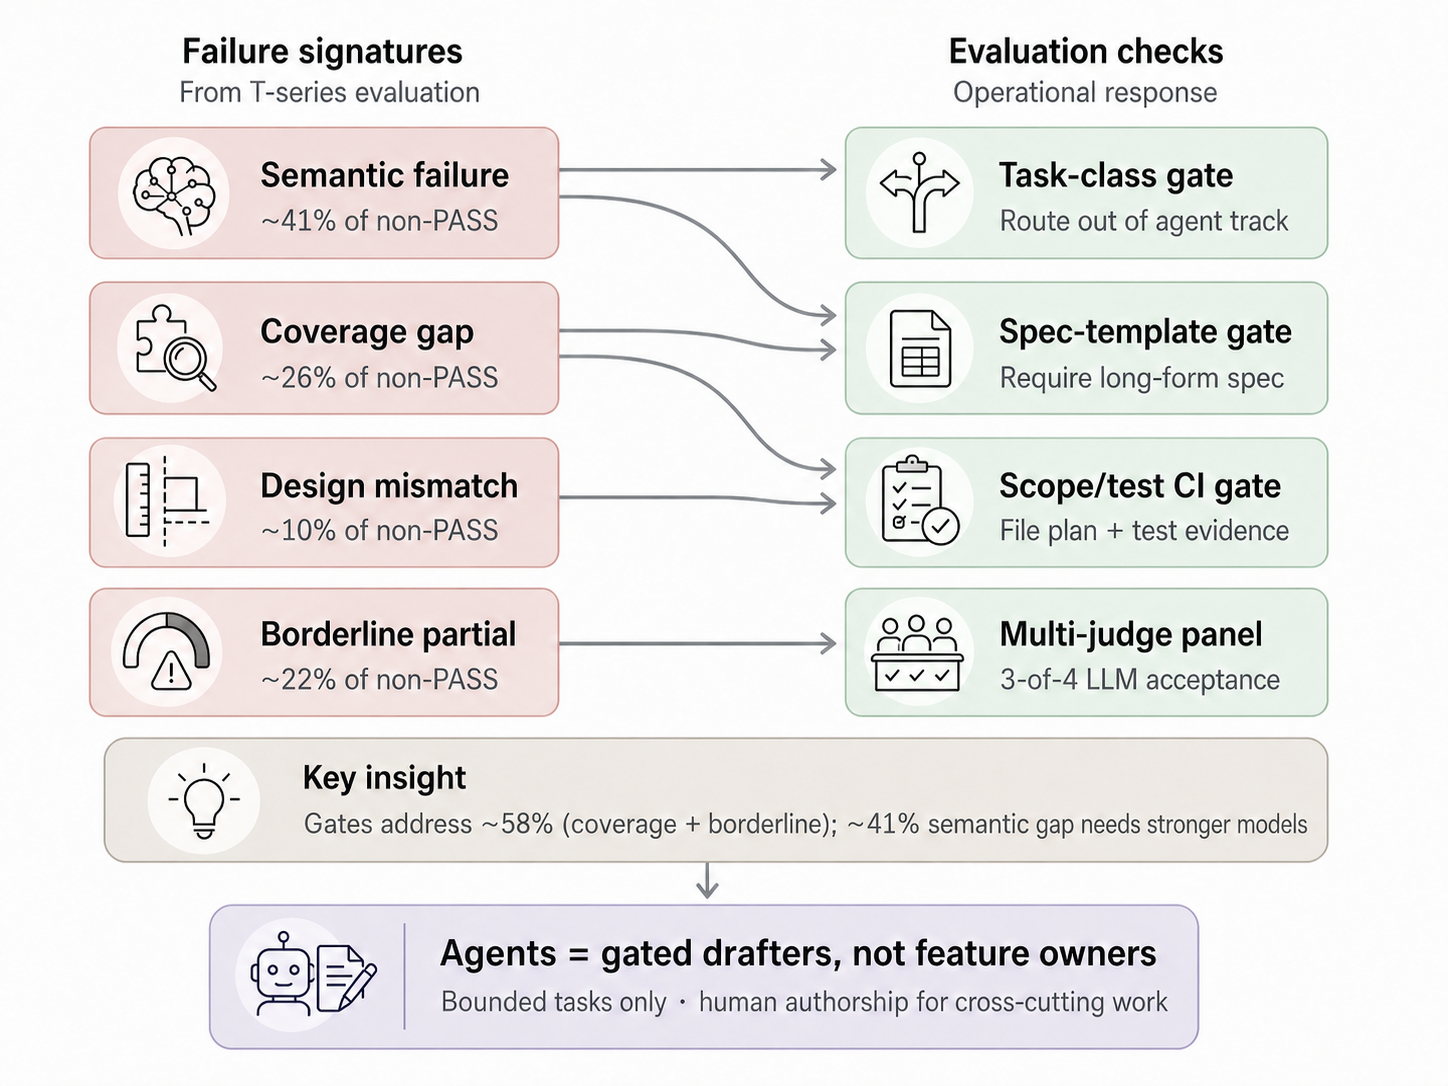
\includegraphics[width=\linewidth]{svg/failure_to_gate_mapping.png}
  \caption{Failure signatures mapped to checks.}
  \label{fig:failure-gate-map}
\end{subfigure}
\caption{From empirical failures to industrial implications. Panel~(a) turns the results into a four-step evaluation workflow: route bounded tasks, require structured specifications, add scope/test checks, and use calibrated multi-evaluator review. Panel~(b) maps failure signatures to the checks most likely to filter them before human review.}
\Description{Two-panel figure. The first panel shows a four-gate workflow for agent use. The second maps semantic failures, coverage gaps, design mismatches, and borderline partials to corresponding checks.}
\label{fig:implication-panels}
\end{figure*}
